\documentclass{article}
\usepackage{tikz}
\usetikzlibrary{positioning}

\begin{document}

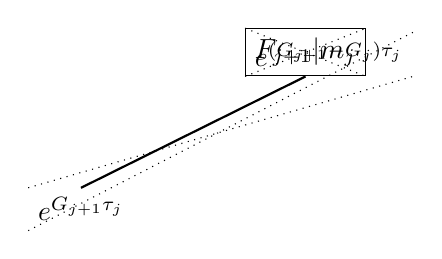
\begin{tikzpicture}[node distance=2cm]
    % Define nodes
    \node (F) [draw] {$F_{j+1}|m_j$};
    \node (G) [below left=of F] {$e^{G_{j+1}\tau_j}$};
    \node (H) [above right=of G] {$e^{(G_{j+1}-G_j)\tau_j}$};

    % Draw the dotted lines
    \draw[dotted] (F.north west) -- (F.south east);
    \draw[dotted] (F.south west) -- (F.north east);
    \draw[dotted] (G.north west) -- (H.south east);
    \draw[dotted] (G.south west) -- (H.north east);

    % Draw the solid line
    \draw[thick] (F.south) -- (G.north);
\end{tikzpicture}

\caption{Computing \( F_{j+1}|m_j \) from \( e^{G_{j+1}\tau_j} \) and \( e^{(G_{j+1}-G_j)\tau_j} \)}

\end{document}